\documentclass[11pt]{article}
\usepackage[a4paper, margin=1.9cm]{geometry}
\usepackage[T1]{fontenc}
\usepackage{lmodern}
\usepackage{microtype}
\usepackage{amsmath, amssymb}
\usepackage{graphicx}
\usepackage{booktabs}
\usepackage{tabularx}
\usepackage{float}
\usepackage{enumitem}
\setlist{itemsep=1pt, topsep=3pt}
\usepackage[font=small, labelfont=bf]{caption}
\usepackage[colorlinks=true, linkcolor=black, citecolor=black, urlcolor=black]{hyperref}

\newcommand{\E}{\mathbb{E}}
\newcommand{\N}{\mathcal{N}}
\newcommand{\xou}{\hat x_0^{\mathrm{OU}}}

\title{Zero-Shot Classifier Guidance via Analytical Ornstein--Uhlenbeck Inversion:\\ Project Report}
\author{Porat Yosef Hai\\[2pt] \small Generative Learning and Diffusion Models (00960236), Technion, Spring 2026}
\date{}

\begin{document}
\maketitle

\begin{abstract}
Training-free guidance steers a pretrained diffusion model with a classifier trained on clean images, by evaluating
the classifier on an estimate of the clean image. TFG~\cite{tfg} unifies these methods; its key component, variance
guidance, differentiates the network's estimate and therefore pays for a backward pass through the network at every
step. We proposed to replace that estimate by the analytical inversion of the forward process,
$\xou = x_t/\sqrt{\bar\alpha_t}$, which needs no backward pass (in continuous time the forward process is the
Ornstein--Uhlenbeck (OU) process, hence the name). On CIFAR-10 label guidance, tested on a single label
(ship), the estimate is cheap but does not guide: 17--22\% accuracy, against 85--90\% for TFG and DPS and 10\% without guidance, and no switch-over point $t^*$
helps. We trace the failure to two causes: the estimate is mostly noise until the last steps, and its Jacobian lacks
the posterior covariance, so the guidance fools the classifier that guides it instead of drawing the object.
\end{abstract}

\section{The proposal}
Training-free guidance needs a clean-image estimate $\hat x_0(x_t)$ at every sampling step, and TFG obtains it from
the diffusion network through Tweedie's formula (Eq.~\eqref{eq:tweedie} below). We propose to obtain it analytically
from the forward process instead:
\begin{itemize}
  \item \textbf{Analytical estimate:} $\xou(x_t) = x_t/\sqrt{\bar\alpha_t}$.
  \item \textbf{Zero backpropagation:} the classifier gradient $\nabla_{x_t}\log p\big(y \mid x_t/\sqrt{\bar\alpha_t}\big)$
        needs only the classifier, not the diffusion network.
  \item \textbf{Threshold:} since dividing by $\sqrt{\bar\alpha_t}$ amplifies the noise variance to
        $(1-\bar\alpha_t)/\bar\alpha_t$, find the threshold $t^*$ beyond which the guidance degrades, and generate
        without guidance there. In the experiments, $t^*$ is the number of final steps that are guided.
  \item \textbf{Evaluation:} compare with TFG in accuracy and quality against computational cost.
\end{itemize}

\section{Background: training-free guidance and its cost}
We use the notation of DDPM and of the paper. One step of the forward process multiplies the image by
$\sqrt{1-\beta_t}$ and adds Gaussian noise of variance $\beta_t$. With $\alpha_t = 1-\beta_t$ and
$\bar\alpha_t = \prod_{s\le t}\alpha_s$, the noisy image at step $t$ is
\begin{equation}\label{eq:forward}
  x_t = \sqrt{\bar\alpha_t}\,x_0 + \sqrt{1-\bar\alpha_t}\;\epsilon, \qquad \epsilon\sim\N(0, I).
\end{equation}
In continuous time this is the OU process $dX_t = -X_t\,dt + \sqrt2\,dW_t$, with $\sqrt{\bar\alpha_t} = e^{-t}$.

\paragraph{Guidance.} To sample from $p_0(x \mid c) \propto p_0(x)\,f_c(x)$, the reverse process needs the conditional
score $\nabla\log p_t(x) + \nabla\log \E[f_c(x_0) \mid x_t = x]$. A classifier trained on noisy images learns the
second term; a training-free method uses a classifier $f$ trained on clean images only, and approximates the term by
$\nabla\log f(x_{0|t})$, where $x_{0|t}$ is Tweedie's estimate from the network $\epsilon_\theta$:
\begin{equation}\label{eq:tweedie}
  x_{0|t} = \frac{x_t - \sqrt{1-\bar\alpha_t}\;\epsilon_\theta(x_t, t)}{\sqrt{\bar\alpha_t}} \;\approx\;
  \E[x_0 \mid x_t] = \frac{x_t + (1-\bar\alpha_t)\,\nabla\log p_t(x_t)}{\sqrt{\bar\alpha_t}}.
\end{equation}

\paragraph{TFG.} TFG~\cite{tfg} writes the existing training-free methods (DPS, LGD, FreeDoM, MPGD and
UGD; see~\cite{tfg} for their references) as special cases of one algorithm with four techniques: variance guidance (the gradient with respect to $x_t$),
mean guidance (the gradient with respect to $x_{0|t}$), smoothing of $f$ with Gaussian noise, and recurrence. A beam
search over three strengths tunes it for each task. Its Lemma~3.3 explains variance guidance: with a perfect network,
\begin{equation}\label{eq:lemma}
  \nabla_{x_t}\log f(x_{0|t}) = \Big(\frac{\partial x_{0|t}}{\partial x_t}\Big)^{\!\top}\nabla_{x_{0|t}}\log f
  = \frac{\sqrt{\bar\alpha_t}}{1-\bar\alpha_t}\,\Sigma_{0|t}\,\nabla_{x_{0|t}}\log f, \qquad
  \Sigma_{0|t} = \mathrm{Cov}[x_0 \mid x_t].
\end{equation}
The covariance moves correlated pixels together and keeps the push along the data, but computing this product requires
a backward pass through the network. Mean guidance avoids it, but alone it is weaker: on CIFAR-10 the paper reports 38\%
for MPGD (mean guidance only) against 50\% for DPS (variance guidance only).

\section{Method: the OU estimate}
Solving Eq.~\eqref{eq:forward} for $x_0$ is exact, but the noise $\epsilon$ is unknown. Tweedie's estimate replaces
it by its posterior mean $\E[\epsilon \mid x_t]$, which is what the network predicts; the OU estimate replaces it by
its prior mean, $\E[\epsilon] = 0$:
\begin{equation}\label{eq:ou}
  \xou = \frac{x_t}{\sqrt{\bar\alpha_t}}.
\end{equation}
Equivalently, $\xou$ is the maximum-likelihood estimate of $x_0$ under
$p(x_t \mid x_0) = \N(\sqrt{\bar\alpha_t}\,x_0, (1-\bar\alpha_t)I)$, or Tweedie's formula without the score term. It
is therefore \emph{not} the posterior mean $\E[x_0 \mid x_t]$: the posterior mean needs the score, which is what the
network provides. Two properties follow.
\begin{itemize}
  \item \textbf{No network.} Its Jacobian is $I/\sqrt{\bar\alpha_t}$, so variance guidance needs no backward pass.
  \item \textbf{Noise.} Substituting Eq.~\eqref{eq:forward},
        $\xou = x_0 + \sqrt{(1-\bar\alpha_t)/\bar\alpha_t}\;\epsilon$, whose noise has variance
        $(1-\bar\alpha_t)/\bar\alpha_t$, as noted in Section~1. With the diffusion model's noise schedule and 100 sampling
        steps, its standard deviation is 157 at the first step and falls below 1, the scale of the pixels, which lie in
        $[-1, 1]$, only in the last 26 steps.
\end{itemize}
Replacing $x_{0|t}$ by $\xou$ in DPS and TFG gives \textbf{OU-DPS} and \textbf{OU-TFG}; everything else stays TFG.
As in the TFG code, both estimates are clipped to $[-1, 1]$ before the classifier. The proposed threshold is tested by
guiding only the last $t^*$ of the 100 steps.

\section{Setup}
We follow the paper's CIFAR-10 label-guidance experiment, on one label (ship).
\begin{itemize}
  \item \textbf{Diffusion model:} \texttt{google/ddpm-cifar10-32}, with 1000 levels and $\beta_t$ linear from $10^{-4}$
        to $0.02$ (the paper's noise schedule).
  \item \textbf{Sampler:} DDIM with 100 steps and $\eta = 1$.
  \item \textbf{TFG settings}, as in the paper's benchmark:
        \begin{itemize}
          \item $N_{\mathrm{recur}} = 1$: each guided step is done once (no recurrence).
          \item $N_{\mathrm{iter}} = 4$: at every sampling step, mean guidance moves the estimate in 4 small gradient
                steps (in the methods that use mean guidance).
          \item ``Increase'' schedule: the strengths grow over the sampling steps, in proportion to $\alpha_t$.
          \item Smoothing: $f$ is evaluated at the estimate plus one sample of Gaussian noise.
        \end{itemize}
  \item \textbf{Strengths:} the three strengths $\bar\rho$ (variance guidance), $\bar\mu$ (mean guidance) and
        $\bar\gamma$ (smoothing) are set by TFG's beam search: start at 0.25 ($\bar\gamma$: 0.001), multiply one strength
        at a time by 2 ($\bar\gamma$: by 10), keep the best two, at most six rounds. Each candidate is scored, as in the
        paper, by the judge's accuracy on 64 images from a different starting noise. The search gave DPS
        $\bar\rho = 0.5$; TFG $(\bar\rho, \bar\mu, \bar\gamma) = (0.5, 0.25, 0.001)$; mean guidance only $\bar\mu = 0.5$,
        $\bar\gamma = 0.01$; OU-DPS $\bar\rho = 0.25$; OU-TFG $(0.25, 0.25, 0.001)$.
  \item \textbf{Classifiers:} the guide is the paper's ResNet-18, which steers the sampling; the judge is an
        independent ConvNeXt-tiny, the paper's evaluator, which never guides.
  \item \textbf{Runs:} 100 images per run, from the same starting noise for every method. Accuracy is the fraction of
        images the judge classifies as ship (one standard error is about 4 points). Time per image and peak GPU memory
        are measured in batches of 100 on a Colab T4 GPU.
\end{itemize}
As a check, our TFG reaches 85\% on ship with $(\bar\rho, \bar\mu, \bar\gamma) = (0.5, 0.25, 0.001)$; the paper
reports 83\% with $(1, 0.25, 0.001)$ (its Table~10).

\section{Results}

\subsection{Cost and accuracy}
Table~\ref{tab:main} and Figure~\ref{fig:accuracy} compare all methods, each guided at every step.

\textbf{Cost.} Without a backward pass, the OU estimate costs about as much as sampling without guidance: OU-DPS takes
0.33\,s per image and 1.6\,GB, close to the 0.26\,s and 1.6\,GB of unguided sampling, while DPS takes 0.72\,s and
5.3\,GB. TFG and OU-TFG are slower than DPS and OU-DPS only because their four mean-guidance steps call the classifier
four more times per step.

\textbf{Accuracy.} The OU estimate does not guide: OU-DPS and OU-TFG reach 22\% and 17\%, barely above the 10\% of
unguided sampling, while DPS and TFG, which use the network's estimate (Tweedie's formula, Eq.~\eqref{eq:tweedie}),
reach 90\% and 85\%. Even mean guidance alone,
which also has no backward pass, does better (34\%).

So the OU estimate is cheap but not accurate: no method reaches the cheap and accurate corner of Figure~\ref{fig:accuracy}
(top left).

\begin{table}[h]
\centering\small
\begin{tabular}{lccccc}
\toprule
method & estimate & backward pass & accuracy & time per image & peak memory \\
\midrule
no guidance        & --      & no  & 10\% & 0.26\,s & 1.6\,GB \\
DPS                & network & yes & 90\% & 0.72\,s & 5.3\,GB \\
TFG                & network & yes & 85\% & 1.03\,s & 5.3\,GB \\
mean guidance only & network & no  & 34\% & 0.55\,s & 1.6\,GB \\
OU-DPS             & OU      & no  & 22\% & 0.33\,s & 1.6\,GB \\
OU-TFG             & OU      & no  & 17\% & 0.72\,s & 1.6\,GB \\
\bottomrule
\end{tabular}
\caption{Label ship, 100 images per run, guided at all 100 steps. Accuracy by the judge; time per image and peak GPU
memory for a batch of 100.}
\label{tab:main}
\end{table}

\begin{figure}[h]
\centering
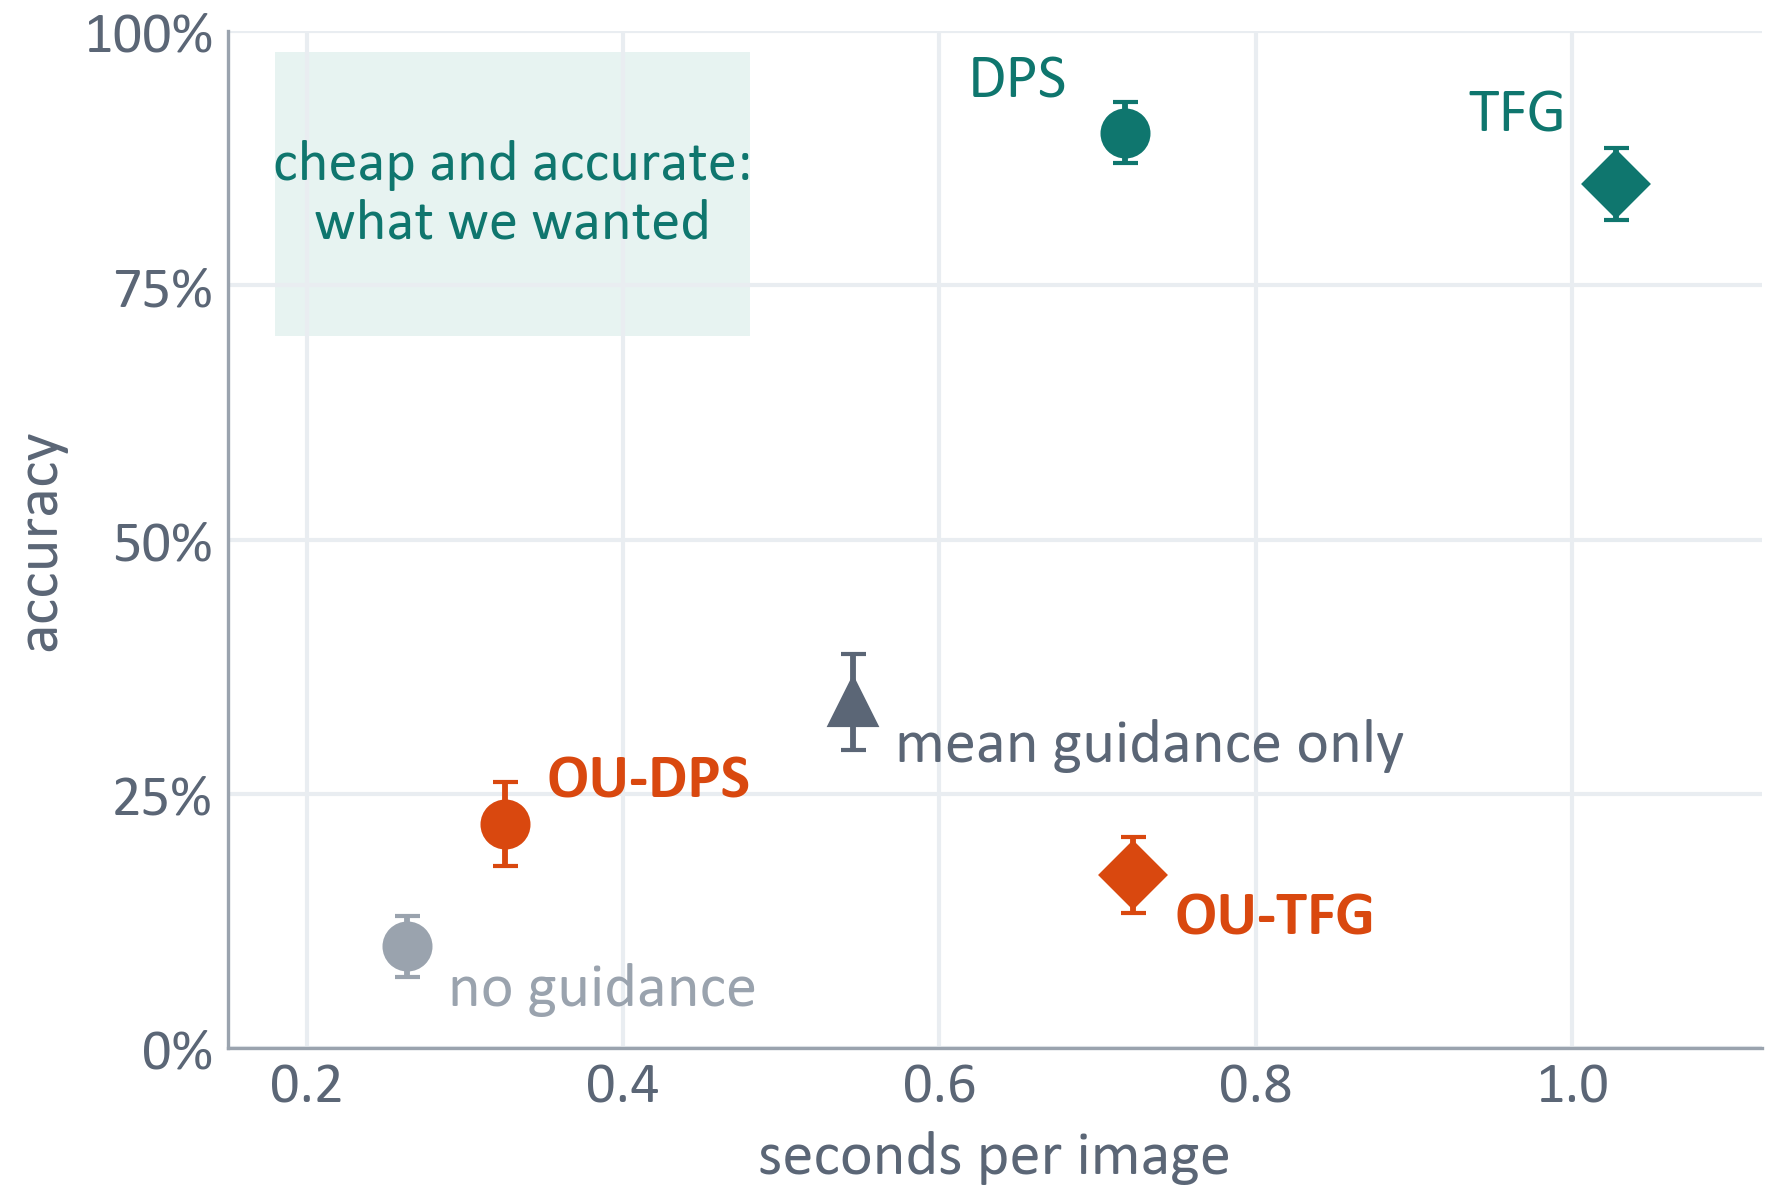
\includegraphics[width=0.4\linewidth]{figures/accuracy_time.png}
\caption{Accuracy against time per image ($\pm$ one standard error). Teal: the network's estimate; orange: the OU
estimate; slate: mean guidance only; gray: no guidance.}
\label{fig:accuracy}
\end{figure}

\subsection{The threshold \texorpdfstring{$t^*$}{t*}}
Guidance through an estimate can only work at the steps where the classifier sees something meaningful in that estimate.
Figure~\ref{fig:threshold} measures where this happens (left), and then tests the proposed threshold (right).

\textbf{Left: when does each estimate show the class?} We sample 64 images \emph{without} guidance and note the class
of each finished image. Then, at every one of the 100 steps, we give each estimate to the guide and check whether it
already predicts that final class. The curve is the fraction of images for which it does.
\begin{itemize}
  \item \textbf{The network's estimate} $x_{0|t}$ (Tweedie's formula, Eq.~\eqref{eq:tweedie}) shows the class from the
        middle of sampling: for 27\% of the images halfway,
        59\% at step 75 and 83\% at step 91.
  \item \textbf{The OU estimate} $\xou$ (Eq.~\eqref{eq:ou}) shows it only at the very end. Its curve is flat at 12.5\%, close to chance (10\%),
        until step 85, and then rises to 36\% at step 96 and 94\% at the last step. Before that, most of its pixels lie
        outside $[-1, 1]$ and are clipped (99.5\% of them at the first step, 76\% halfway), so the guide sees an almost
        saturated image.
\end{itemize}

\textbf{Right: guiding only the last $t^*$ steps.} Since the OU estimate is informative only near the end, the
proposed threshold suggests using it only there: we guide with it in the last $t^*$ steps and sample without guidance
before them. For every $t^*$ from 5 to 100, the accuracy stays between 12\% and 27\%.

\textbf{Conclusion.} The network's estimate shows that the class of the image is decided around the middle of
sampling. After that, the remaining steps add little noise and change the image only slightly, so the guidance can no
longer turn it into a different class. The OU estimate becomes informative only in these last steps, when it is too
late to change the class, so no threshold helps.

\begin{figure}[h]
\centering
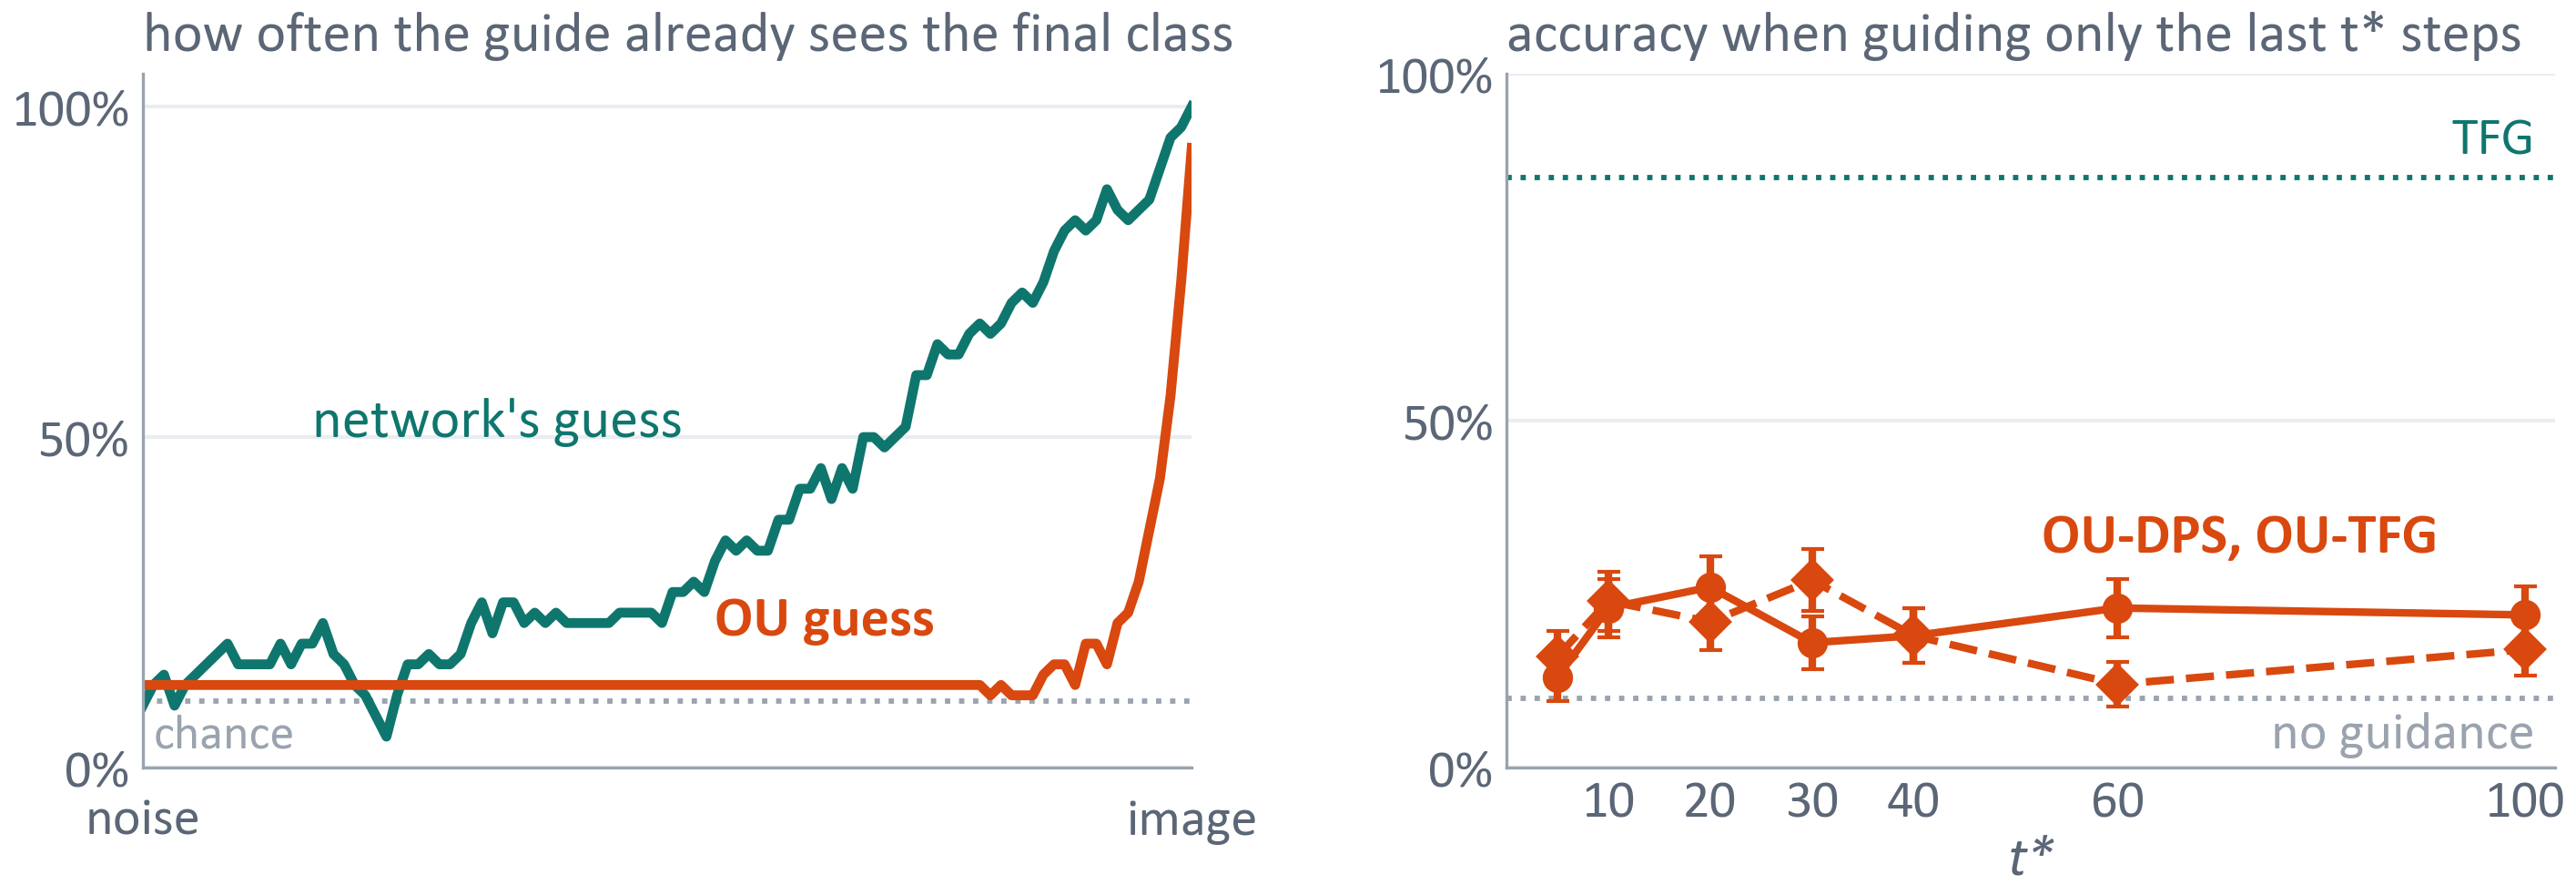
\includegraphics[width=0.8\linewidth]{figures/where_useful.png}
\caption{Left: sampling without guidance; how often the guide sees the final class in each estimate. Right: accuracy
when guiding with the OU estimate only in the last $t^*$ steps (100 images per run).}
\label{fig:threshold}
\end{figure}

\subsection{Why it fails: the guide is fooled}
A guided image can get a high score from the guiding classifier without showing the object: the guidance may only
exploit weaknesses of that classifier. We therefore scored the same 64 images of each run with both classifiers, the
guide, which steered the sampling, and the judge, which did not (Figure~\ref{fig:judge}, left).
\begin{itemize}
  \item \textbf{With the network's estimate} they agree: the guide calls 100\% of the images ship, and the judge
        89--91\%.
  \item \textbf{With the OU estimate} they disagree: the guide calls 97--100\% of the images ship, but the judge only
        17--20\%, even though the strengths were chosen to maximize the judge's accuracy (Section~4).
  \item \textbf{Mean guidance alone} is fooled as well: 100\% against 36\%.
\end{itemize}
The images (Figure~\ref{fig:judge}, right) show why. From the same starting noise, TFG draws ships, while OU-DPS keeps
the unguided image and paints colored patterns on it: the guidance raised the guide's score without drawing a ship.

\begin{figure}[h]
\centering
\begin{minipage}[c]{0.38\linewidth}\centering
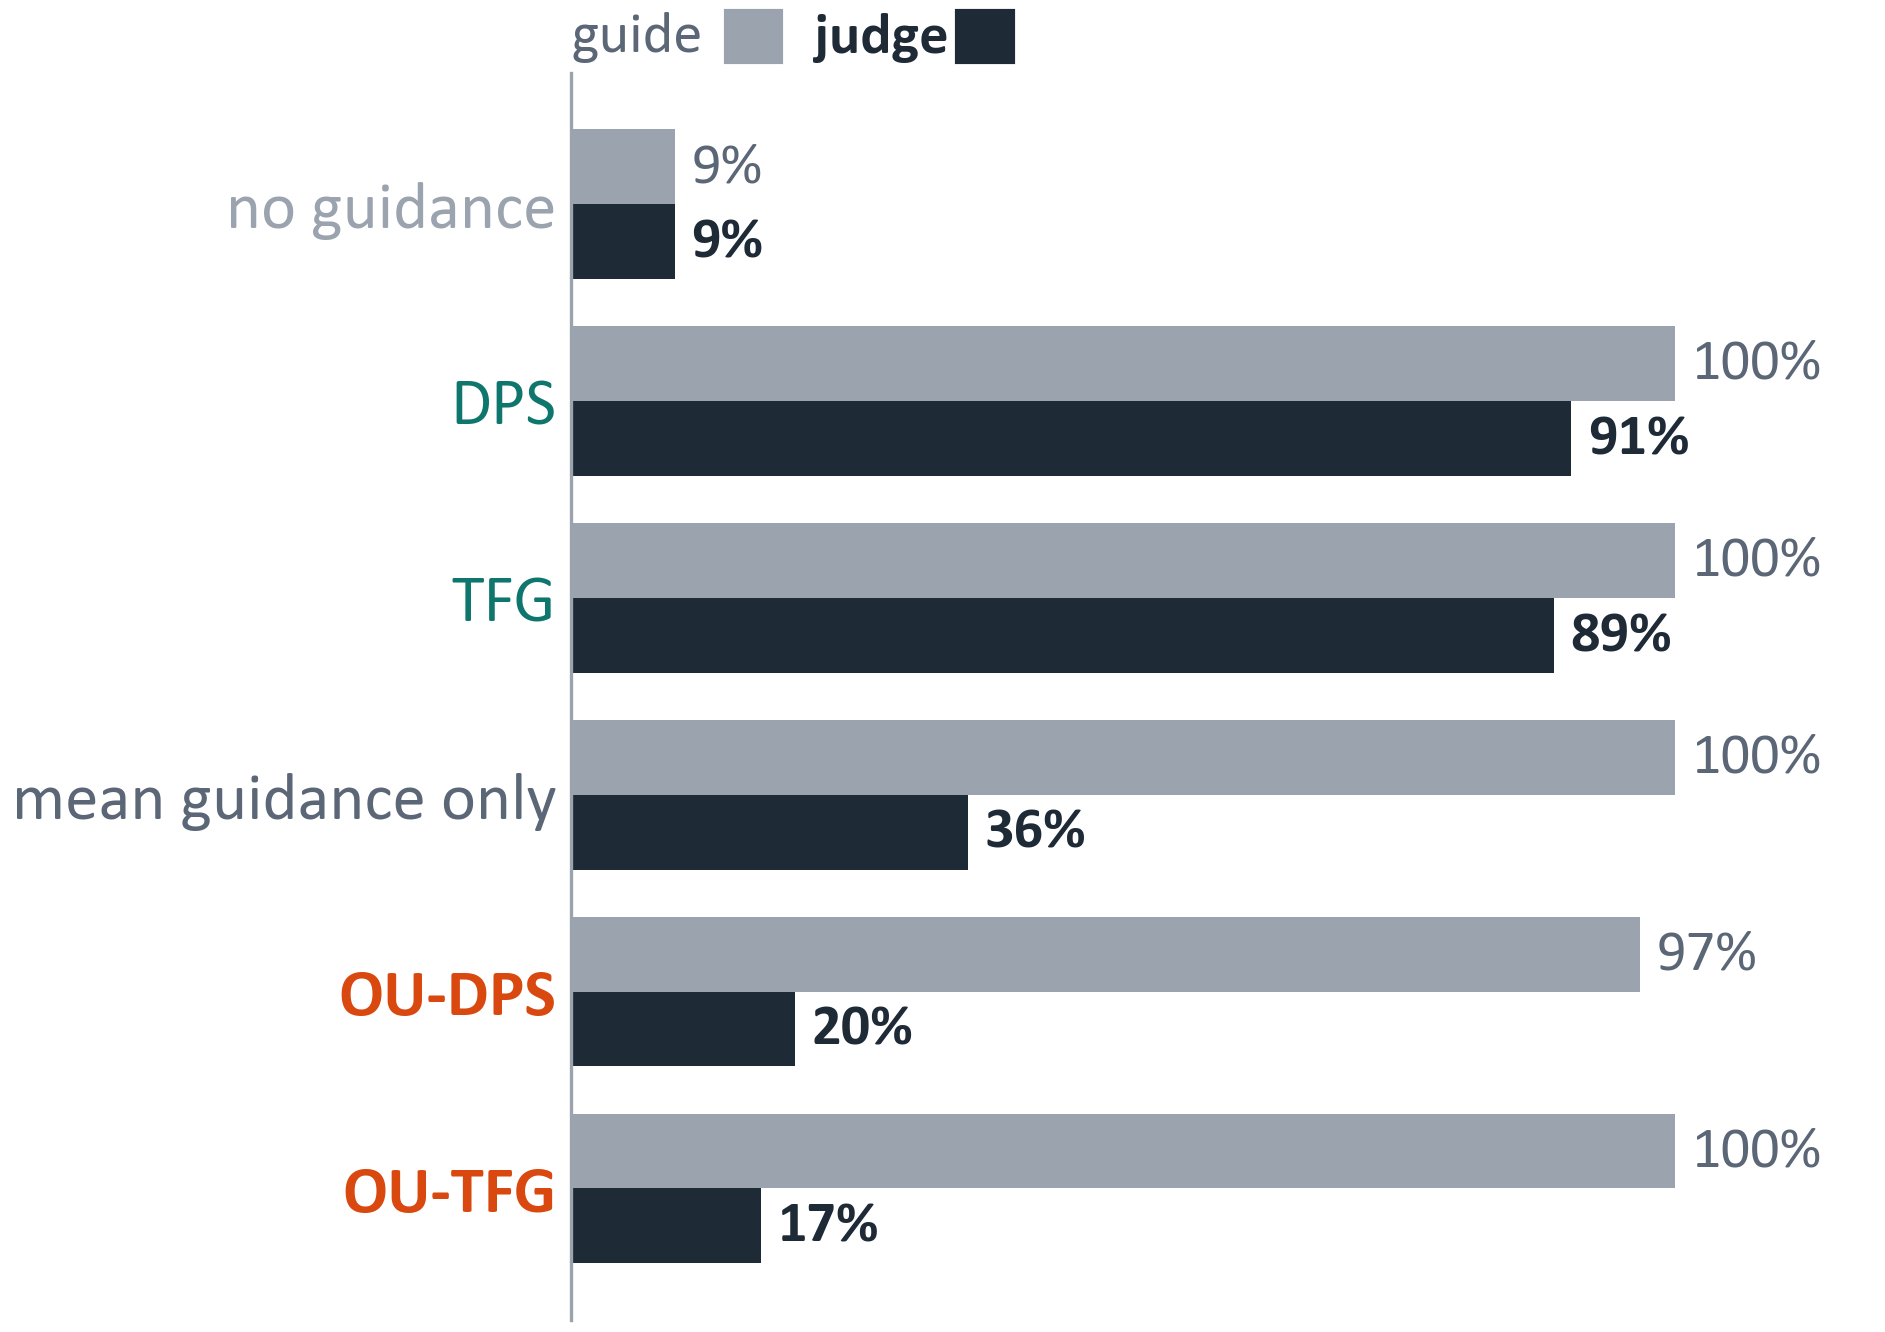
\includegraphics[width=\linewidth]{figures/guide_judge.png}
\end{minipage}\hfill
\begin{minipage}[c]{0.5\linewidth}\centering
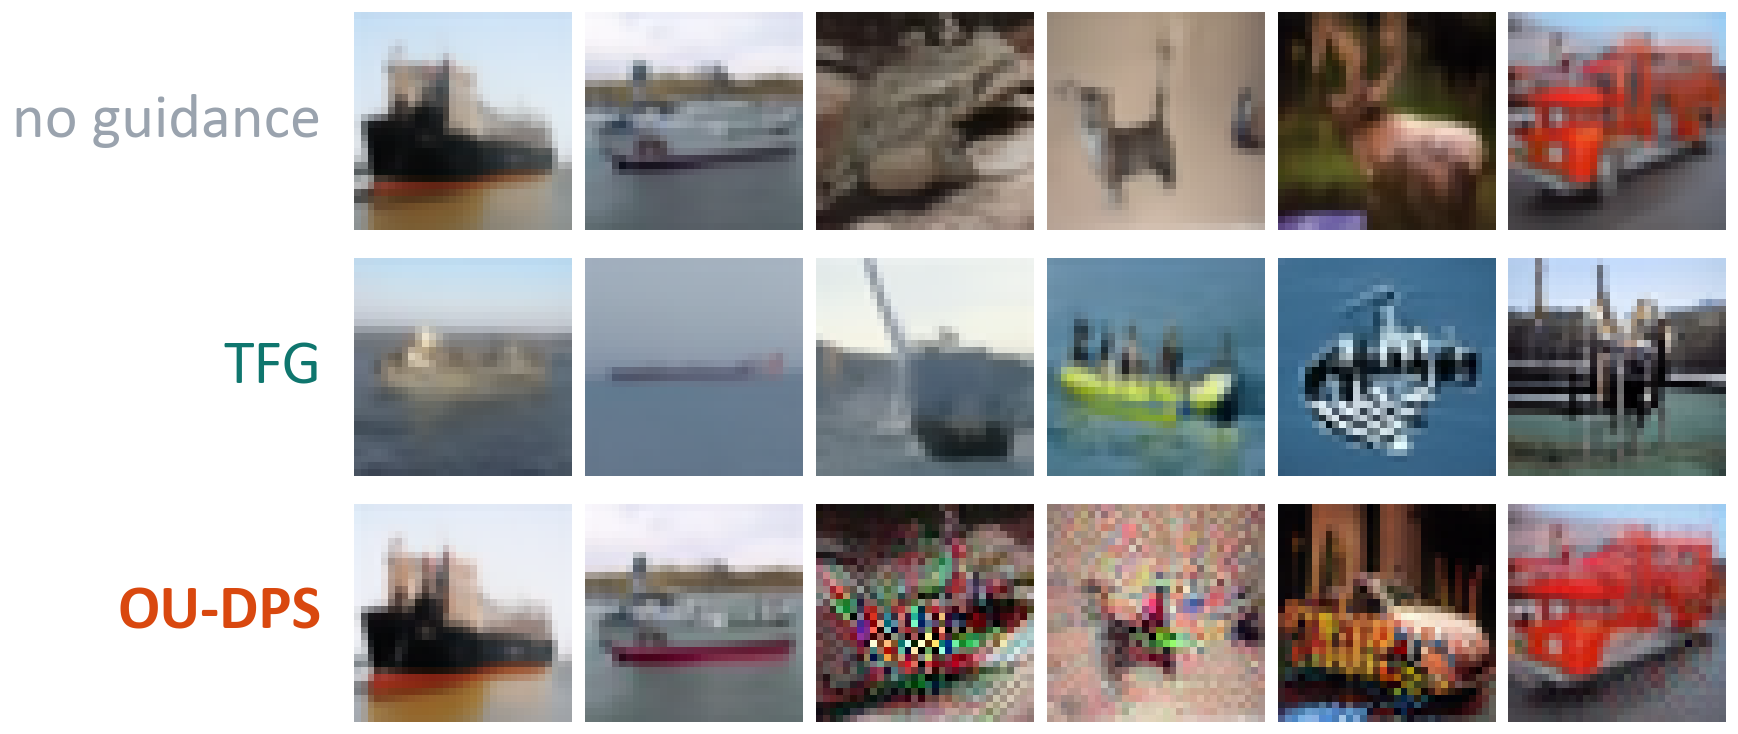
\includegraphics[width=\linewidth]{figures/samples.png}
\end{minipage}
\caption{Left: the fraction of the same 64 images called ship by the guide (gray) and by the judge (dark). Right: each
column starts from the same noise.}
\label{fig:judge}
\end{figure}

\textbf{The explanation}, which we worked out after these results, has two parts.
\begin{itemize}
  \item \textbf{Noise.} Until the last steps, the OU estimate is mostly noise and mostly clipped (Section~3), which
        explains Section~5.2.
  \item \textbf{No covariance.} By Eq.~\eqref{eq:lemma}, variance guidance through the network's estimate multiplies
        the classifier's gradient by the posterior covariance, which moves correlated pixels together and keeps the
        change along the data. Through the OU estimate it multiplies it by $I/\sqrt{\bar\alpha_t}$ instead, so the raw
        gradient of the classifier reaches every pixel independently. This is the classic recipe for adversarial
        examples: it raises the classifier's score with small patterns rather than with an object. Mean guidance also
        applies the raw gradient, which is why it is fooled too.
\end{itemize}

\subsection{TFG then OU}
Section~5.2 showed that the OU estimate is informative only in the last steps. A natural compromise is therefore to let
TFG guide while the class is being decided, and to switch to the cheap OU estimate only at the end: TFG for the first
$100-k$ steps, and OU guidance (with strengths searched for each $k$) in the last $k$ steps. To see whether the OU
estimate contributes anything there, a control run switches the guidance off in the last $k$ steps instead
(Figure~\ref{fig:tfgou}).
\begin{itemize}
  \item \textbf{Up to $k = 20$} both keep TFG's accuracy (85\%) within the noise: 87\% ($k = 10$) and 80\% ($k = 20$)
        with the OU estimate, 81\% and 80\% without guidance. Both save 10--20\% of the backward passes.
  \item \textbf{For larger $k$} both drop, because TFG no longer guides the steps in which the class is decided: at
        $k = 60$, 39\% with the OU estimate and 28\% without guidance.
  \item \textbf{On average over $k$}, the OU estimate adds 5 points over the control, within the noise of 100 images.
\end{itemize}
\textbf{Conclusion.} The saving is real, but it comes from the last steps barely needing guidance, not from the OU
estimate: the last 10--20\% of TFG's steps can run without guidance at almost no loss.

\begin{figure}[h]
\centering
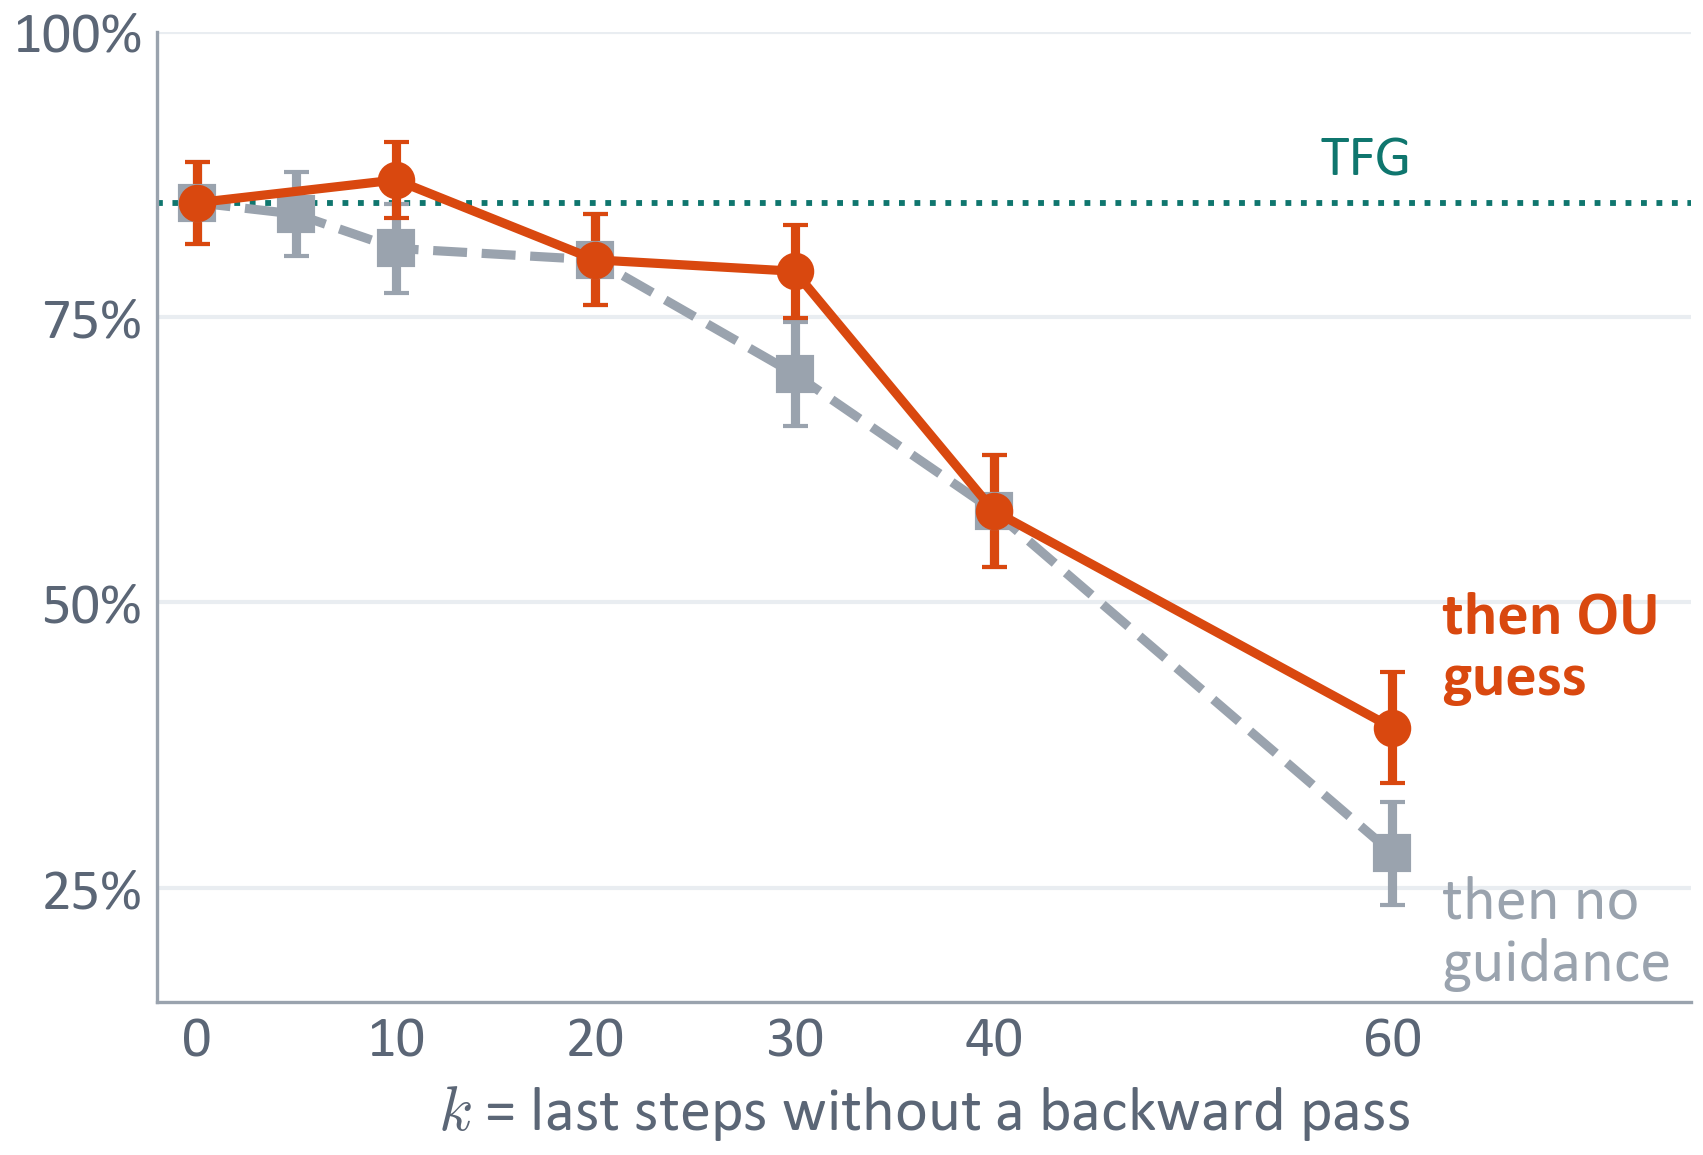
\includegraphics[width=0.36\linewidth]{figures/tfg_then_ou.png}
\caption{Accuracy against $k$, the number of final steps without a backward pass ($\pm$ one standard error).}
\label{fig:tfgou}
\end{figure}

\section{Conclusion and limitations}
The OU estimate removes the backward pass of training-free guidance, but it cannot replace the network's estimate. The
backward pass pays for the posterior covariance of Lemma~3.3, and the guidance needs it: without the covariance, the
guidance fools the classifier that guides it instead of drawing the object, and the estimate becomes informative only
after the class has been decided. Along the way, TFG and DPS were reproduced (85\% on ship, against 83\% in the paper),
and the last 10--20\% of TFG's steps were found to barely need guidance, a free saving. In addition, we
diagnosed both estimates step by step during sampling, tested the guide against an independent judge, and combined TFG
with the OU estimate against a control.

\textbf{Limitations.} The experiments cover one task and one label (ship, an easy one), whereas the paper averages over
ten labels. Each run has only 100 images, so every accuracy has a standard error of about 4 points: small differences
between methods are not meaningful, while large ones, such as 85\% against 20\%, are. For the same reason, the image quality (FID) is
not reported: with 100 images per run it is strongly biased.

\begingroup\small
\begin{thebibliography}{9}\setlength{\itemsep}{0pt}
\bibitem{tfg} H.~Ye, H.~Lin, J.~Han, et al. TFG: Unified training-free guidance for diffusion models. \emph{NeurIPS},
2024.
\end{thebibliography}
\endgroup

\end{document}
